\documentclass[12pt,a4paper]{article}
\usepackage{color}
\usepackage{colortbl}
\usepackage{amsmath}
\usepackage{amssymb}
\usepackage[colorinlistoftodos,textsize=scriptsize]{todonotes}

\begin{document}

	 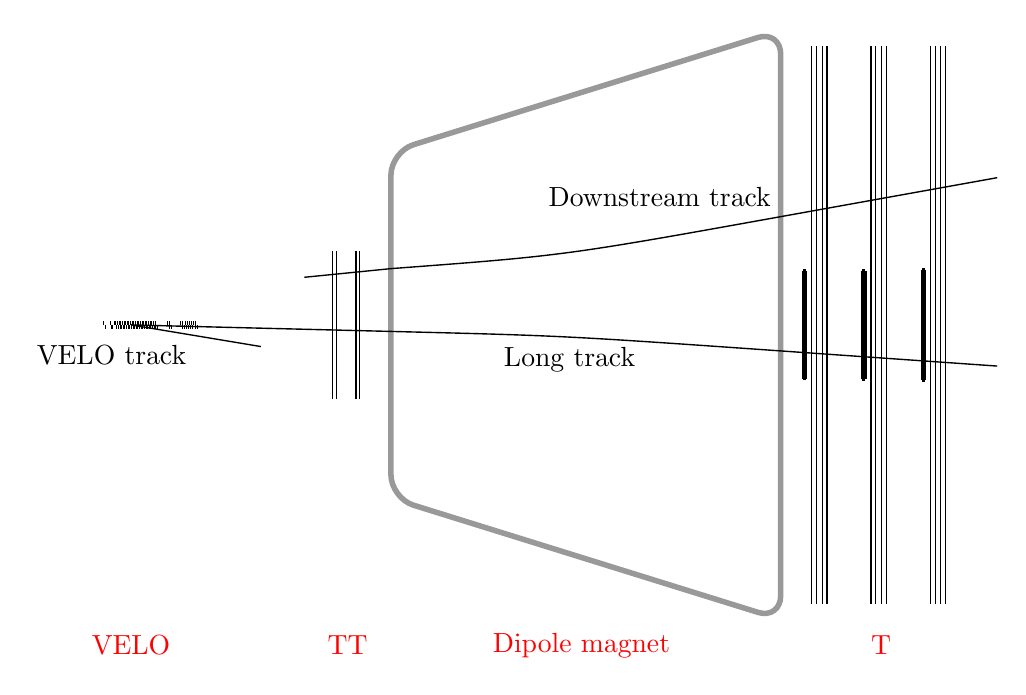
\begin{tikzpicture}[scale=.11]
	   \tikzset{
  veloStation/.style={double, double distance=.1mm}
, puStation/.style={}
, ttLayer/.style={}
, magnet/.style={line width=2pt,draw=black!40!white,rounded corners=3mm}
, itLayer/.style={}
, otLayer/.style={}
, rich/.style={draw=none,fill=green!40!white}
, spd/.style={draw=none,fill=blue!40!white}
, converter/.style={draw=none,fill=green!40!white}
, prs/.style={draw=none,fill=yellow!40!white}
, ecal/.style={draw=none,fill=orange!40!white}
, hcal/.style={draw=none,fill=yellow!40!white}
, muon/.style={draw=none,fill=red!40!white}
}

% VELO
\draw[veloStation] (-17.5mm,-0.2mm) -- (-17.5mm,5.0mm);
\draw[veloStation] (-14.5mm,-0.2mm) -- (-14.5mm,5.0mm);
\draw[veloStation] (-11.5mm,-0.2mm) -- (-11.5mm,5.0mm);
\draw[veloStation] (-8.5mm,-0.2mm) -- (-8.5mm,5.0mm);
\draw[veloStation] (-5.5mm,-0.2mm) -- (-5.5mm,5.0mm);
\draw[veloStation] (-2.5mm,-0.2mm) -- (-2.5mm,5.0mm);
\draw[veloStation] (0.5mm,-0.2mm) -- (0.5mm,5.0mm);
\draw[veloStation] (3.5mm,-0.2mm) -- (3.5mm,5.0mm);
\draw[veloStation] (6.5mm,-0.2mm) -- (6.5mm,5.0mm);
\draw[veloStation] (9.5mm,-0.2mm) -- (9.5mm,5.0mm);
\draw[veloStation] (12.5mm,-0.2mm) -- (12.5mm,5.0mm);
\draw[veloStation] (15.5mm,-0.2mm) -- (15.5mm,5.0mm);
\draw[veloStation] (18.5mm,-0.2mm) -- (18.5mm,5.0mm);
\draw[veloStation] (21.5mm,-0.2mm) -- (21.5mm,5.0mm);
\draw[veloStation] (24.5mm,-0.2mm) -- (24.5mm,5.0mm);
\draw[veloStation] (27.5mm,-0.2mm) -- (27.5mm,5.0mm);
\draw[veloStation] (43.5mm,-0.2mm) -- (43.5mm,5.0mm);
\draw[veloStation] (58.5mm,-0.2mm) -- (58.5mm,5.0mm);
\draw[veloStation] (63.5mm,-0.2mm) -- (63.5mm,5.0mm);
\draw[veloStation] (68.5mm,-0.2mm) -- (68.5mm,5.0mm);
\draw[veloStation] (73.5mm,-0.2mm) -- (73.5mm,5.0mm);
\draw[veloStation] (-16.0mm,0.2mm) -- (-16.0mm,-5.0mm);
\draw[veloStation] (-13.0mm,0.2mm) -- (-13.0mm,-5.0mm);
\draw[veloStation] (-10.0mm,0.2mm) -- (-10.0mm,-5.0mm);
\draw[veloStation] (-7.0mm,0.2mm) -- (-7.0mm,-5.0mm);
\draw[veloStation] (-4.0mm,0.2mm) -- (-4.0mm,-5.0mm);
\draw[veloStation] (-1.0mm,0.2mm) -- (-1.0mm,-5.0mm);
\draw[veloStation] (2.0mm,0.2mm) -- (2.0mm,-5.0mm);
\draw[veloStation] (5.0mm,0.2mm) -- (5.0mm,-5.0mm);
\draw[veloStation] (8.0mm,0.2mm) -- (8.0mm,-5.0mm);
\draw[veloStation] (11.0mm,0.2mm) -- (11.0mm,-5.0mm);
\draw[veloStation] (14.0mm,0.2mm) -- (14.0mm,-5.0mm);
\draw[veloStation] (17.0mm,0.2mm) -- (17.0mm,-5.0mm);
\draw[veloStation] (20.0mm,0.2mm) -- (20.0mm,-5.0mm);
\draw[veloStation] (23.0mm,0.2mm) -- (23.0mm,-5.0mm);
\draw[veloStation] (26.0mm,0.2mm) -- (26.0mm,-5.0mm);
\draw[veloStation] (29.0mm,0.2mm) -- (29.0mm,-5.0mm);
\draw[veloStation] (45.0mm,0.2mm) -- (45.0mm,-5.0mm);
\draw[veloStation] (60.0mm,0.2mm) -- (60.0mm,-5.0mm);
\draw[veloStation] (65.0mm,0.2mm) -- (65.0mm,-5.0mm);
\draw[veloStation] (70.0mm,0.2mm) -- (70.0mm,-5.0mm);
\draw[veloStation] (75.0mm,0.2mm) -- (75.0mm,-5.0mm);
% PU
\draw[puStation] (-31.5mm,-0.2mm) -- (-31.5mm,5.0mm);
\draw[puStation] (-23.5mm,-0.2mm) -- (-23.5mm,5.0mm);
\draw[puStation] (-30.0mm,0.2mm) -- (-30.0mm,-5.0mm);
\draw[puStation] (-22.0mm,0.2mm) -- (-22.0mm,-5.0mm);

%% RICH1

% TT
\draw[ttLayer] (232.75mm,-85.6mm) -- (232.75mm,85.6mm);
\draw[ttLayer] (237.25mm,-85.6mm) -- (237.25mm,85.6mm);
\draw[ttLayer] (259.75mm,-85.6mm) -- (259.75mm,85.6mm);
\draw[ttLayer] (264.25mm,-85.6mm) -- (264.25mm,85.6mm);

% MAGNET -- BY HAND
\draw[magnet] (300.mm,200.mm) -- (750.mm,340.mm) -- (750.mm,-340.mm) -- (300.mm,-200.mm) -- cycle;

% IT
\draw[itLayer] (775.5mm,-62.1mm) -- (775.5mm,62.1mm); %/dd/Structure/LHCb/AfterMagnetRegion/T/IT/Station1/CSideBox/LayerX1
\draw[itLayer] (776.9mm,-64.1mm) -- (776.9mm,64.1mm); %/dd/Structure/LHCb/AfterMagnetRegion/T/IT/Station1/CSideBox/LayerU
\draw[itLayer] (778.8mm,-64.1mm) -- (778.8mm,64.1mm); %/dd/Structure/LHCb/AfterMagnetRegion/T/IT/Station1/CSideBox/LayerV
\draw[itLayer] (780.3mm,-62.1mm) -- (780.3mm,62.1mm); %/dd/Structure/LHCb/AfterMagnetRegion/T/IT/Station1/CSideBox/LayerX2
\draw[itLayer] (843.7mm,-62.8mm) -- (843.7mm,62.8mm); %/dd/Structure/LHCb/AfterMagnetRegion/T/IT/Station2/CSideBox/LayerX1
\draw[itLayer] (845.1mm,-64.8mm) -- (845.1mm,64.8mm); %/dd/Structure/LHCb/AfterMagnetRegion/T/IT/Station2/CSideBox/LayerU
\draw[itLayer] (847.0mm,-64.8mm) -- (847.0mm,64.8mm); %/dd/Structure/LHCb/AfterMagnetRegion/T/IT/Station2/CSideBox/LayerV
\draw[itLayer] (848.5mm,-62.8mm) -- (848.5mm,62.8mm); %/dd/Structure/LHCb/AfterMagnetRegion/T/IT/Station2/CSideBox/LayerX2
\draw[itLayer] (912.2mm,-63.5mm) -- (912.2mm,63.5mm); %/dd/Structure/LHCb/AfterMagnetRegion/T/IT/Station3/CSideBox/LayerX1
\draw[itLayer] (913.6mm,-65.5mm) -- (913.6mm,65.5mm); %/dd/Structure/LHCb/AfterMagnetRegion/T/IT/Station3/CSideBox/LayerU
\draw[itLayer] (915.5mm,-65.5mm) -- (915.5mm,65.5mm); %/dd/Structure/LHCb/AfterMagnetRegion/T/IT/Station3/CSideBox/LayerV
\draw[itLayer] (917.0mm,-63.5mm) -- (917.0mm,63.5mm); %/dd/Structure/LHCb/AfterMagnetRegion/T/IT/Station3/CSideBox/LayerX2

% OT
\draw[otLayer] (786.080130227mm,-322.0mm) -- (786.080130227mm,322.0mm);
\draw[otLayer] (791.530094892mm,-322.0mm) -- (791.530094892mm,322.0mm);
\draw[otLayer] (798.080196464mm,-322.0mm) -- (798.080196464mm,322.0mm);
\draw[otLayer] (803.530161128mm,-322.0mm) -- (803.530161128mm,322.0mm);
\draw[otLayer] (854.280588294mm,-322.0mm) -- (854.280588294mm,322.0mm);
\draw[otLayer] (859.730552959mm,-322.0mm) -- (859.730552959mm,322.0mm);
\draw[otLayer] (866.280654531mm,-322.0mm) -- (866.280654531mm,322.0mm);
\draw[otLayer] (871.730619195mm,-322.0mm) -- (871.730619195mm,322.0mm);
\draw[otLayer] (922.781008406mm,-322.0mm) -- (922.781008406mm,322.0mm);
\draw[otLayer] (928.230973071mm,-322.0mm) -- (928.230973071mm,322.0mm);
\draw[otLayer] (934.781110653mm,-322.0mm) -- (934.781110653mm,322.0mm);
\draw[otLayer] (940.231075317mm,-322.0mm) -- (940.231075317mm,322.0mm);

%% the track types

\tikzset{track/.style={line width=.5pt}}
% Velo
\draw[track] (0mm,0mm) -- node[below left] {VELO track} (150mm,-25mm);
% Upstream
% T
% Downstream
\draw[track] (200mm,55mm) -- (300mm,65mm) .. controls (500mm,80mm) .. (750mm,125mm) node[above left] {Downstream track} -- (1000mm,170mm);
% Long
\draw[track] (0mm,0mm) -- (300mm,-7.5mm) .. controls (500mm,-12.5mm) .. node[below] {Long track} (750mm,-30mm) -- (1000mm,-47.5mm);

\node[red] at (0,-370mm) {VELO};
\node[red] at (250mm,-370mm) {TT};
\node[red] at (520mm,-370mm) {Dipole magnet};
\node[red] at (866mm,-370mm) {T};
 	 \end{tikzpicture}

\end{document}